\chapter{Introduction}

Here we introduce and familiarise with the basic definitions and notations about Cellular Automata, a tool dating back to the late 1940s, when Stanislaw Ulam and John von Neumann defined it as a model for natural and biological processes.

\section{Cellular Automaton}
\label{ca}

A cellular automaton (abbrev. CA) is a discrete dynamical system consisting of cells that change their states simultaneously according a local update rule. This update process is repeated at discrete time steps.
Cellular automata are\cite{canotes}

\begin{itemize}
	\item discrete in space and time,
	\item homogeneous in space and time,
	\item local in their interactions.
\end{itemize}


\paragraph{Basics}

Let:

\begin{itemize}

	\item $\mathds{Z}^{d}$ be a $d$-dimensional cellular space, with $d \in \mathds{N}^{+}$. Elements of this set are called \textit{cells}.

	\item $S$ be a finite state set. Elements of this set are called \textit{states}.

	\item $c$ be a \textit{configuration} of a d-dimensional CA with a state set S, defined as the following function:

	$$c: \mathds{Z}^d \rightarrow S$$
	that assigns a state to each cell.

	\item $c(\vec{n })$ the state of a cell $\vec{n} \in \mathds{Z}^d$

\end{itemize}

Most frequently we consider one and two-dimensional spaces, in which cases the cells from a line are indexed by $\mathds{Z}$ (line) or by $\mathds{Z}^2$ (grid).

Denoting the set of functions from set A from B with $B^A$ we can write that the set of all configurations is $S^{\mathds{Z}^d}$.

A d-dimensional neighborhood vector of size m is a tuple

$$N = N = (\vec{n}_1,\vec{n}_2,...,\vec{n}_m) $$

where each $\vec{n}_i \in \mathds{Z}^d$ and $\vec{n}_i \neq \vec{n}_j$ for all $i \neq j$.

The \textit{local update rule} of a CA with state set S and size m neighborhood is a fuction

$$ f: S^m \rightarrow S$$

specifying the new state of the cell based on the old states of its neighborhood.

As we mentioned, all cells use the same rule, and this rule is applied simultaneously. Global configuration $c$ becomes $c'$ where for all $\vec{n} \in \mathds{Z}^n$:

$$c'(\vec{n}) = f[c(\vec{n}, \vec{n}_1),c(\vec{n}, \vec{n}_2), ... , c(\vec{n}, \vec{n}_m)]$$

$c \mapsto c' $ is our \textit{global transition function} $G: S^{\mathds{Z}^d} \longrightarrow S^{\mathds{Z}^d}$. Typically, G is iterated to produce a time evolution of the system.

$$ c \mapsto G(c) \mapsto G^2(c) \mapsto G^2(c) \mapsto..$$

\paragraph{Formal definition}

A CA is a 4-tuple $A=(d, S,N,f)$ where

\begin{itemize}
	\item d is the dimension,
	\item S is the finite state set,
	\item N is the neighborhood vector,
	\item f is the local update rule.
\end{itemize}

\subsection{Neighborhoods}

\begin{figure*}
  \centering
  \subfigure[Von Neumann]{%
    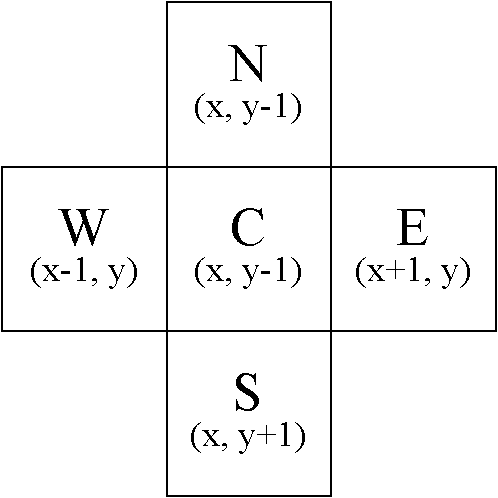
\includegraphics[width=0.4\textwidth]{vn_n}%
    \label{fig:a}%
    }\hspace{1cm}%or more
    \subfigure[Moore]{%
    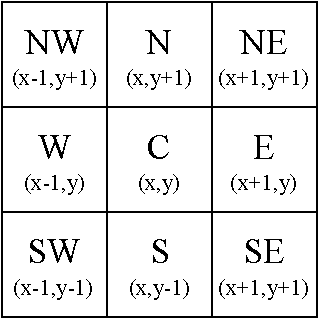
\includegraphics[width=0.4\textwidth]{m_n}%
    \label{fig:b}%
    
  }%  
  \caption{Moore and Von Neumann neighborhoods for Cellular Automata}
  \label{fig:2d_n}
\end{figure*}

\begin{figure*}
  \centering
    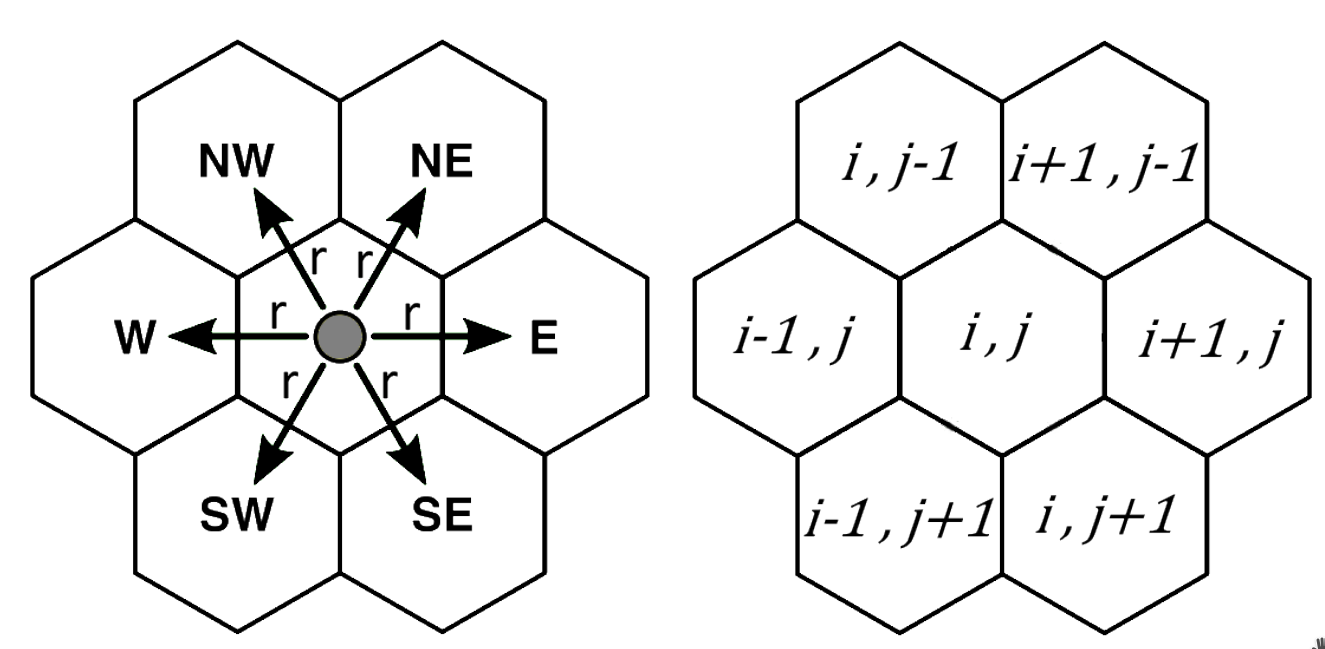
\includegraphics[width=0.8\textwidth]{hex_n}%
    
  \caption{Hexagonal neighborhod for Cellular Automata\cite{hex_phy}}
  \label{fig:hex_n}
\end{figure*}

When considering two-dimensional CA, the \textit{von Neumann} and the \textit{Moore} neighborhoods (pictured in figure \ref{fig:2d_n}) are often used.

\paragraph{Moore neighborhood}

The d-dimensional radius-r Moore neighboorhood, containing $(2r +1)^d$ elements is defined as follows:

$$M_r^d = (k_1, K_2,...,k_d) \in \mathds{Z}^d \text{ where } |k_i| \leq r \text{  } \forall i = 1,2,...,d $$ 

\paragraph{Von Neumann neighboorhood}


$$V_r^d = (k_1, K_2,...,k_d) \in \mathds{Z}^d \text{ where } \sum_{i=1}^{d} |k_i| \leq r$$



\subsection{Examples}

\begin{figure*}
  \centering
    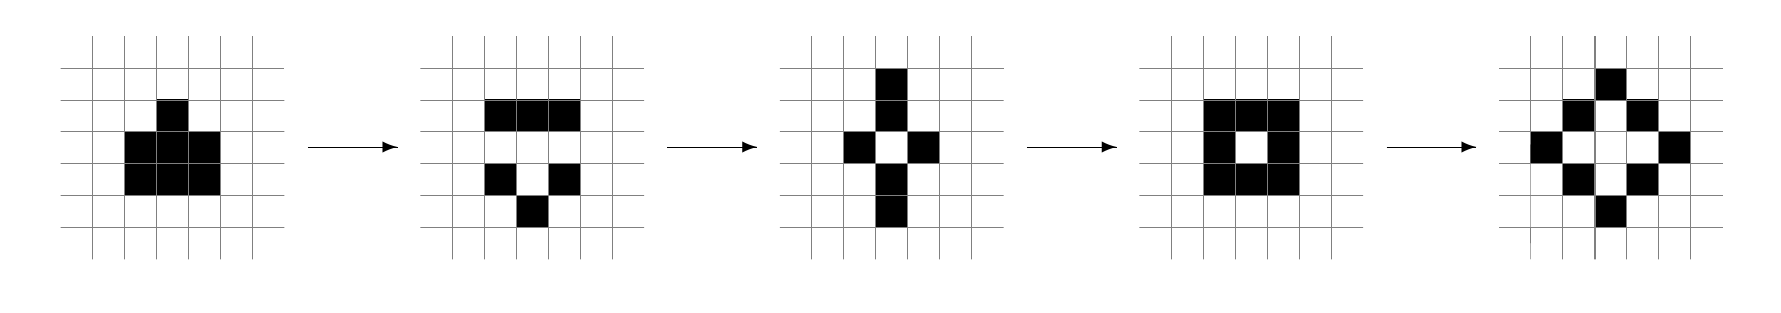
\includegraphics[width=1\textwidth]{gameoflife_example}%
    
  \caption{Five steps of a time evolution in Conway's Game-of-life\cite{canotes}}
  \label{fig:gameoflife}
\end{figure*}


\par
The most known CA in the scientific literature is \textit{Game of Life}, devised by the John Horton Conway in 1970 with the intention of producing a simple model of von Neumann's idea of the machine capable of reproducing itself and simulate a Turing machine. 
\par
In the universe of \textit{Game of Life} each cell is in one of two possible states, alive or dead (or populated and unpopulated, respectively). Every cell interacts with its eight neighbours, which are the cells that are horizontally, vertically, or diagonally adjacent. At each step in time, the following transitions occur:
\begin{itemize}
	\item Any live cell with fewer than two live neighbours dies, as if by underpopulation
	\item Any live cell with two or three live neighbours lives on to the next generation
	\item Any live cell with more than three live neighbours dies, as if by overpopulation
	\item Any dead cell with exactly three live neighbours becomes a live cell, as if by reproduction
\end{itemize}
\par
The initial pattern constitutes the seed of the system. The first generation is created by applying the above rules simultaneously to every cell in the seed; births and deaths occur simultaneously, and the discrete moment at which this happens is sometimes called a tick. Each generation is a pure function of the preceding one. The rules continue to be applied repeatedly to create further generations. 

\section{Physarum}
Physarum polycephalum \cite{sun2017physarum}, \cite{mayne2016biology} is a species of order Physarales, subclass Myxogas-tromycetidae, class Myxomecetes, division Myxostelida, commonly known as a true slime mould.
It is a single celled protist that is visible to the naked eye. Slime mold inhabits shady, cool and moist areas that exist on decaying leaves and logs in forest areas.
\par
It exhibits a very wide repertoire of pattern formation behaviors used for growth, movement, food foraging, nutrient transport, hazard avoidance, and shape maintenance. 
\par
Physarum thrives in favorable environmental conditions, particularly when the right combinations of humidity, temperature and nutrient presence are found. If the conditions are not adequate for development, Physarum behaves like a single-celled organism that does not demonstrate organizational skills. In appropriate conditions, it joins together to create particularly efficient filamentary nets in physical distribution.

\subsection{Life Cycle}
Spores, released from mature fruiting bodies, germinate into mononuclear amoebae (n), which propagate by mitosis. At high population density, amoebae are able to mate, to form a zygote (2n). This diploid cell later develops into a multinuclear plasmodium (2n), through multiple nuclear divisions. Following starvation, the plasmodium can be induced to sporulation by visible light. Later, the plasmodial mass develops into individual fruiting bodies, which will subsequently yield haploid spores (n) \cite{physlf}.

\begin{figure*}
  \centering
    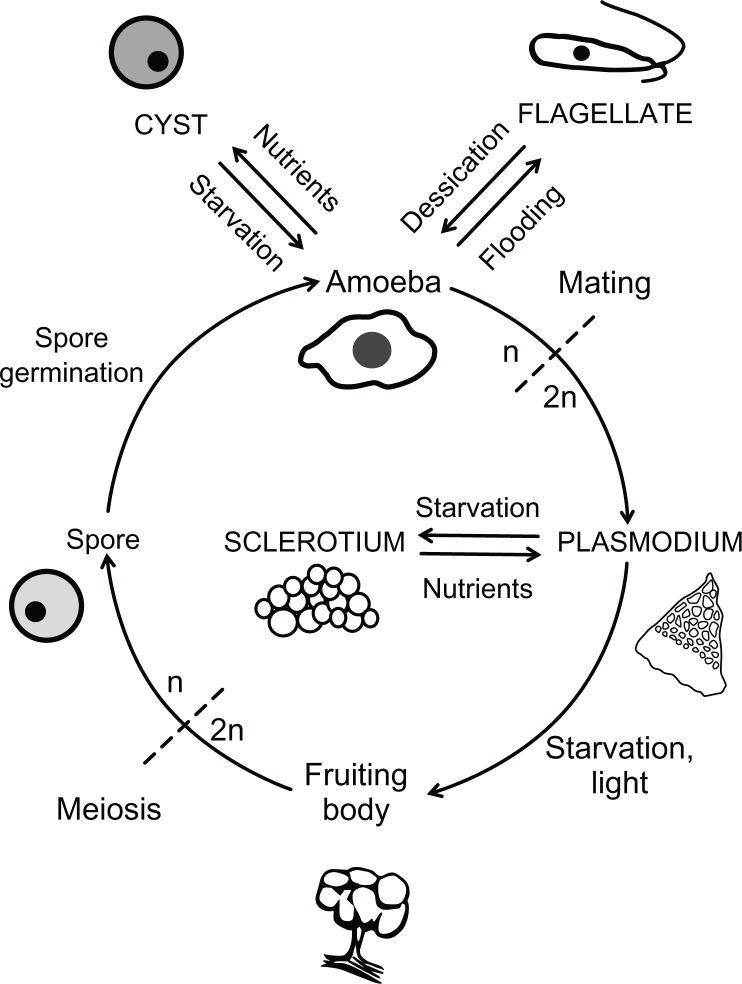
\includegraphics[width=0.8\textwidth]{physarum_life_cycle}%
    
  \caption{The life cycle of Physarum polycephalum\cite{physlf}}
  \label{fig:physarum_life_cycle}
\end{figure*}


It is common to refer to the Physarum by the name of its vegetative (resting) life cycle phase, the plasmodium. The Physarum plasmodium is a single yellow cytoplasmic mass that can range in size from a few mm$^2$ to over half a m$^2$. The organism will typically be composed of a network of protoplasmic veins that can contain more than 100,000 nuclei.
\par
It is during this stage that the organism searches for food. Multiple sources state that the plasmodium is both predatory and saprophytic: its natural foodstuffs include fungal spores, bacteria, smaller amoebae and decaying matter, the latter of which may be digested extracellularly through the secretion of enzymes.

\par
To find its prey, slime mould is able to explore its environment by spontaneous and self-organised oscillatory contractions \cite{jones2015exploiting}. This means that the slime mould is able to contract its body in an organized way, allowing the organism to slowly push itself in all directions. When a slime mould encounters a new food source, it is able to connect the new food source to its pre-existing ones. To conserve mass, the slime mould gradually funnels the link between the food sources to a single protoplasmic tube.
 
\begin{figure*}
  \centering
    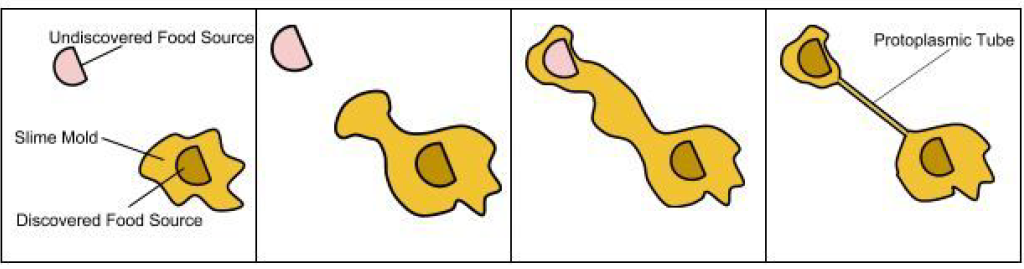
\includegraphics[width=0.8\textwidth]{phys_tubecreation}%
    
  \caption{Physarum protoplasmic tube formation}
  \label{fig:phys_tubecreation}
\end{figure*}

\par
This protoplasmic tube has the ability to exchange not only nutrients, but also information throughout the entire network the slime mold creates. This allows the slime mould to conduct a logical and efficient search of its surroundings to decide what the most efficient method of utilizing its resources is.
In early stages of slime mold development, the Physarum exists in a feeding phase, in which the slime mold remains on an already discovered food source, and increases in mass. The organism will then gradually transition into a more explorative phase, where it discovers new sources of food and prepares to create fruiting bodies, which eventually create more slime mould.
\par
If environmental conditions cause the plasmodium to desiccate during feeding or migration, Physarum will have another life cycle phase called the sclerotium. The sclerotium is basically highly resistant desiccated tissue that serves as a dormant stage, protecting Physarum for long periods of time. The organism will assume it if environmental conditions become too
unfavourable. Once favorable conditions resume, a sclerotium can be revert back to a viable plasmodium that reappears to continue its quest for food.
\par
As the food supply runs out, the plasmodium stops feeding and begins its reproductive phase. Stalks of sporangia form from the plasmodium. It is within these structures that meiosis occurs and spores are formed. Sporangia are usually formed in the open spaces so that the spores they release will be spread by wind currents.
\par
Spores can remain dormant for years if needed. However, when environmental conditions are favorable for growth, the spores germinate and release either flagellated or amoeboid swarm cells (motile stage). The swarm cells then fuse together to form a new plasmodium. 

\par
DA INTEGRARE? 
\par
The plasmodium is an aggregate of protoplasm with a network of tubular elements through which nutrients and chemical signals circulate, the geometry of which is related to internal communication. Moreover, the tubes act as "legs", allowing the organism to navigate around its environment, and can be disassembled and reassembled within a few hours in response to changes in external conditions \cite{nakagaki2004obtaining}.


\par
DA INTEGRARE? 
\par
This, in turn, drives tip growth in the direction of the highest nutrient density by initiating pseudopodium formation (directed actin cytoskeleton assembly, membrane synthesis, etc.). Plasmodial sensing is continuous, pan-directional, and multisensorial (optical, temperature, etc.) and the actions of  each receptor occur concurrently.
Via the combined action of amoeboid tip-growth and contraction of muscle proteins which shuttle the contents of the cytoplasm in the direction of movement, the plasmodium forms a network of tubular structures between all NSs, as illustrated in Figure 2, which typically assumes a highly optimised topology. When being at rest, the fluid contents of  the cytoplasm oscillate rhythmically, distributing internalised food, organelles, and intraplasmodial chemical signalling compounds.Thus, fluid movements within the plasmodium are subjected to dynamically optimizing alternations.


\par
DA INTEGRARE? 
\par
The plasmodium of Physarum is a membrane-bound syncytium of nuclei within a cytoplasm composed of a complex gel-sol network. The gel phase is composed of a spongelike matrix of contractile actin and myosin fibers through which the protoplasmic sol flows. Local oscillations in the thickness of the plasmodium spontaneously appear with approximately 2-min duration. The spatial and temporal organization of the oscillations has been shown to be extremely complex and affects the internal movement of sol through the network by assembly and disassembly of the local actin-myosin structures. The protoplasm moves backward and forward within the plasmodium in a characteristic manner known as shuttle-streaming.
The plasmodium is able to sense local concentration gradients, and the presence of nutrient gradients appears to alter the structure of external membrane areas. The softening of the outer membrane causes a flux of protoplasm in the general direction of the gradient in response to internal pressure changes caused by the local thickness oscillations. The strong coupling between membrane contraction and streaming movement is caused by the incompressibility of the fluid, requiring a constant volume—the weakening of the membrane provides an outlet for the pressure. When the plasmodium has located and engulfed nearby food sources, protoplasmic veins appear within the plasmodium, connecting the food sources. The veins transport protoplasm among the distributed extremes of the organism.
The relative simplicity of the cell and the distributed nature of its control system make Physarum a suitable subject for research into distributed computation substrates. \cite{jones2010characteristics}

The mechanisms used to fulfil these requirements are growth, movement, and area reduction. During the growth-and-foraging stage the plasmodium exhibits a default, broadly reticulated outward growth patter - albeit one that is influenced by substrate and gradient quality. Once nutrients have been located, the topology of the pattern is influenced by the nutrient distribution - the connectivity patterns (the protoplasmic tube network) evolve to achieve a compromise between minimal transport costs and
fault tolerance. Since the plasmodium obviously cannot have any global knowledge about the initial or optimal topology, the network must evolve by physical forces acting on the protoplasmic transport.




